\documentclass {article} 
\usepackage [spanish] {babel}
\usepackage[scaled]{uarial}
\usepackage{color}
\renewcommand*\familydefault{\sfdefault}
\usepackage[T1]{fontenc}
\usepackage [utf8x]{inputenc}
\usepackage{graphicx}
\usepackage[table,usenames,dvipsnames]{xcolor}
\usepackage{hyperref}
\hypersetup{colorlinks,
    citecolor=black,
    filecolor=black,
    linkcolor=black,
    urlcolor=black}
\usepackage{anysize}
\marginsize{1cm}{1cm}{1cm}{2cm}
\usepackage{fancyhdr}
\usepackage{lscape}

\begin{document} 

%\section{Portada}
	\thispagestyle{empty}

\begin{minipage}{0.20\textwidth}
	
\includegraphics[width=0.5\textwidth]{cover/ipn.jpg}
\end{minipage}
\begin{minipage}{0.60\textwidth}
\begin{center}
\LARGE Instituto Politécnico Nacional \newline
\LARGE Escuela Superior de Cómputo \newline
\LARGE Academia de Ingeniería de Software \newline
\end{center}
\end{minipage}
\begin{minipage}{0.20\textwidth}

\includegraphics[width=0.8\textwidth]{cover/escom.jpg}

\end{minipage}%

\vspace{3cm}
\centerline{\huge Análisis del Proyecto }
\vspace{0.3cm}
\centerline{\huge \bf Buscador de Oferta Laboral TI}

\vspace{2cm}

\centerline{\Large  M. en C. Tanibet Pérez de los Santos Mondragón }
\vspace{2cm}
\centerline{\Large  Segundo Parcial }

\vspace{2cm}

\centerline{\Large \bf Integrantes Equipo 10}
\vspace{0.6cm}
\centerline{\Large  David Hernández Muñoz}
\vspace{0.6cm}
\centerline{\Large  Luis Gerardo Heras Hernández}
\vspace{0.6cm}
\centerline{\Large  Alberto Xavier Gómez Ponce}
\vspace{0.6cm}
\centerline{\Large  Sergio Guerra Vega}

\vspace{0.8cm}

\centerline{\Large \bf Grupo }
\vspace{0.6cm}
\centerline{\Large  3CV7 }

\vspace{2cm}
{\large  M\'{e}xico, D.F. \hfill 2013}

\newpage

%-------------------------
\setlength{\headheight}{15pt}
\pagestyle{fancy}
\fancyhf{}
\lhead{
	\begin{tabular}{|l|p{13.3cm}|} 
	\hline
		\cellcolor{Black}\textcolor{White}{\textbf{Web Application Development}} & Análisis del Proyecto\\ 
	\hline
		\cellcolor{Black}\textcolor{White}{\textbf{Fecha}} & \today \\ 
	\hline
		\multicolumn{2}{|c|}{\cellcolor{Black}\textcolor{White}{\textbf{Buscador de Oferta Laboral TI}}}
	\end{tabular}
}
\lfoot{Web Application Development, Análisis del Proyecto}
\rfoot{ Página \thepage} 
%-------------------------

.\linebreak
\tableofcontents
\listoffigures
\listoftables

\newpage

\section{Introducción}
\frame
{
  \frametitle{Introducción} 
 Las búsquedas de empleo por Internet pueden ser una pérdida de tiempo si no se cuenta con las herramientas adecuadas, además de que la mayoría de las vacantes que se presentan no son actuaes o bien pueden tratarse de estafas.
\newline
Nuestro sistema es una alternativa a la búsqueda de empleo tradicional, las búsquedas electrónicas actualmente facilitan muchas de  las actividades cotidianas, buscar empleo no es la excepción,  "Buscador de Oferta Laboral TI"  será un sistema de  fácil uso pero de gran potencia para la vinculación Empleado-Empleador. 
}
\frame
{
\frametitle{Descripci\'on del funcionamiento del sistema}
	
	\subsection{Descripción del funcionamiento del sistema}

\begin{enumerate}
	\item Las empresas podrán crear perfiles y así mismo vacantes para que los aplicantes puedan solicitar el puesto que más les interese. Además las empresas podrán conocer a los aplicantes, sus capacidades y su CV, y así decidir por el que más les convenza. 
	\item El administrador del sistema podrá administrar a las empresas y a los aplicantes que se hayan registrado en el sistema, y después de investigarlos, darlos de baja del sistema si es que se trata de una empresa que no exista o de algún aplicante que no sea real. 
\end{enumerate}

}

\frame
{
\frametitle{Descripci\'on del funcionamiento del sistema}
	\subsection{Descripción del funcionamiento del sistema}

\begin{enumerate}
	

	\item El sistema determinara que vacantes y en que empresas esta más capacitado el aplicante dependiendo sus aptitudes y habilidades.
	\item Los aplicantes podrán ver los vacantes en la página principal del sistema de las empresas que se hayan registrado y si los aplicantes ya se encuentra registrados podrán contactar con la empresa y andarles su CV para que estas los revisen. 
\end{enumerate}

}


\newpage
\section{Diagrama de Casos de Uso}
\frame
{
  \frametitle{Diagrama de Casos de Uso}
  
\begin{figure}[h]
\begin{center}
	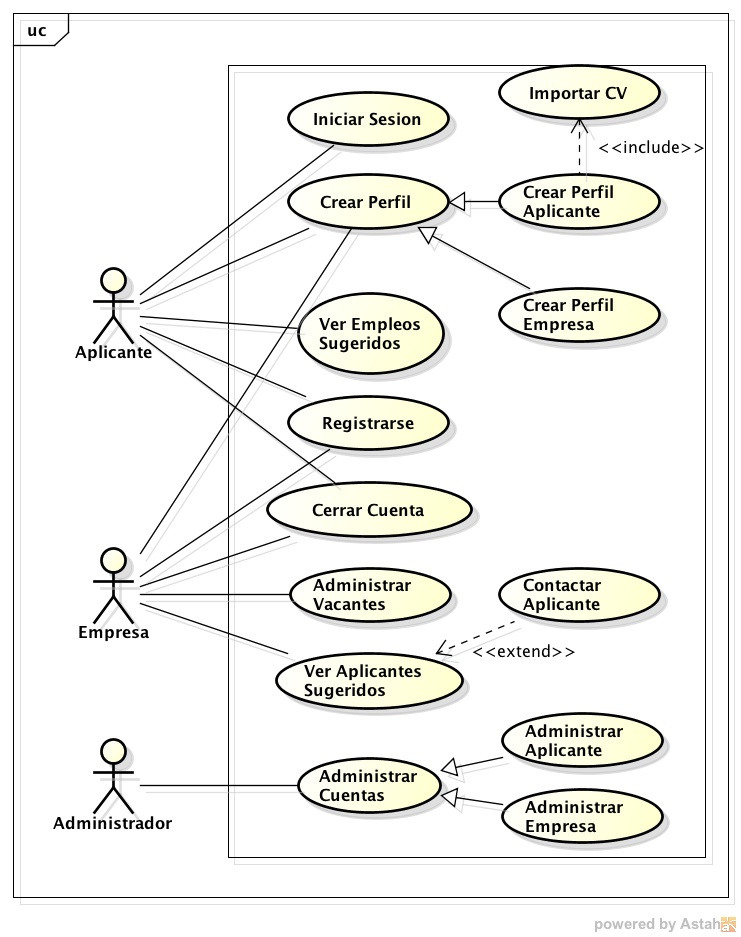
\includegraphics[scale=0.3]{./resources/Modelo_de_Caosos_de_Uso.png}
	\caption{Diagrama de Casos Usos}
	\label{fig:usercasediagram}
\end{center}
\end{figure}

}
\newpage
\section{Diagrama de Actividades}

\begin{figure}[h]
\begin{center}
	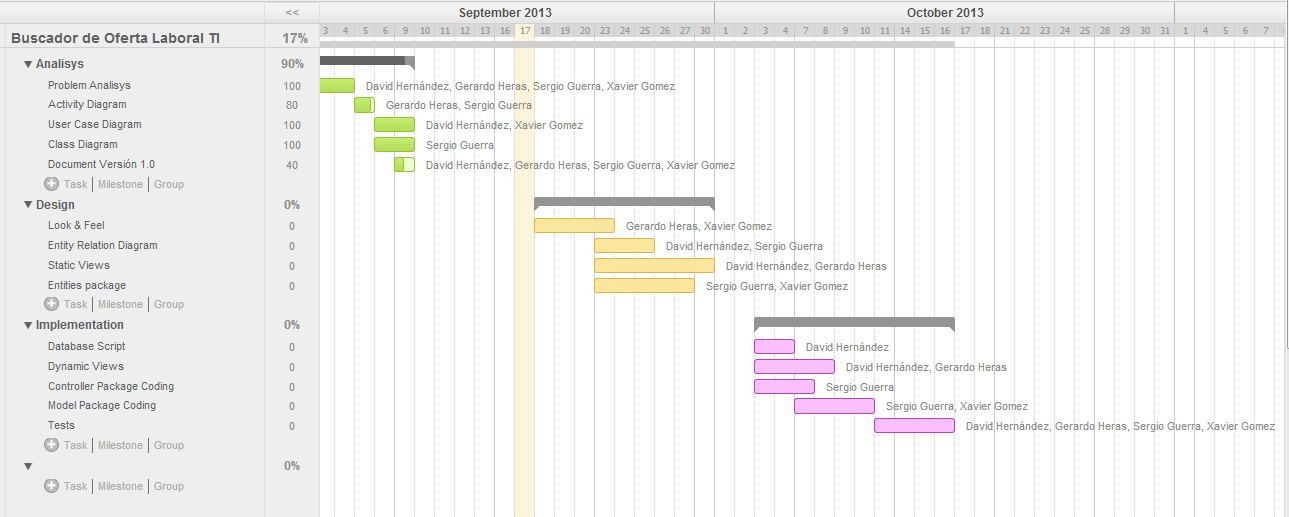
\includegraphics[scale=0.55]{./resources/ActDiagram.png}
	\caption{Diagrama de Actividades}
	\label{fig:actdiagram}
\end{center}
\end{figure}
\newpage
\newpage
\section{Diagrama de Clases}
\subsection{Arquitectura}
\frame
{
  \frametitle{Diagrama de Clases}
  \begin{center}
		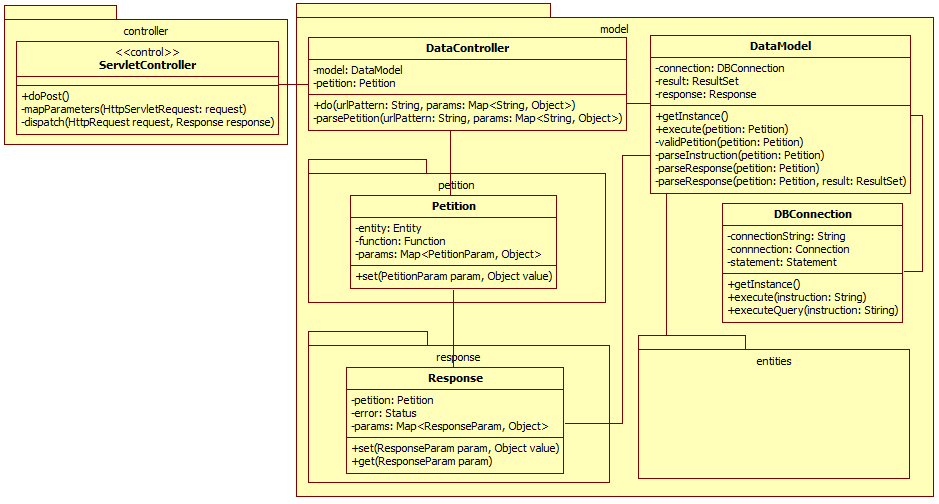
\includegraphics[scale=0.42]{./resources/ClassDiagramArchitecture.png}
  \end{center}
}
\subsection{Entidades}
\frame
{
  \frametitle{Diagrama de Clases}
  \begin{center}
		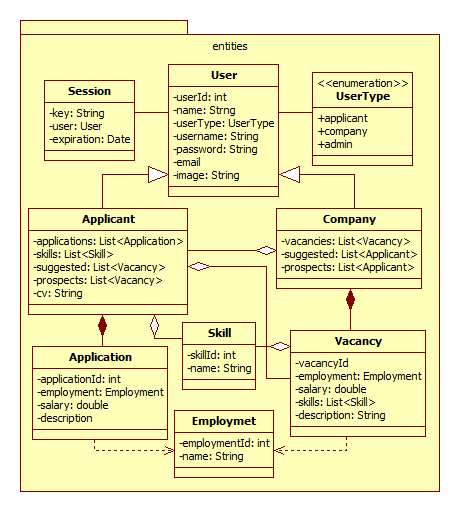
\includegraphics[scale=0.47]{./resources/ClassDiagramEntities.png}
  \end{center}
}
\subsection{Petición / Respuesta}
\frame
{
  \frametitle{Diagrama de Clases}
  \begin{center}
		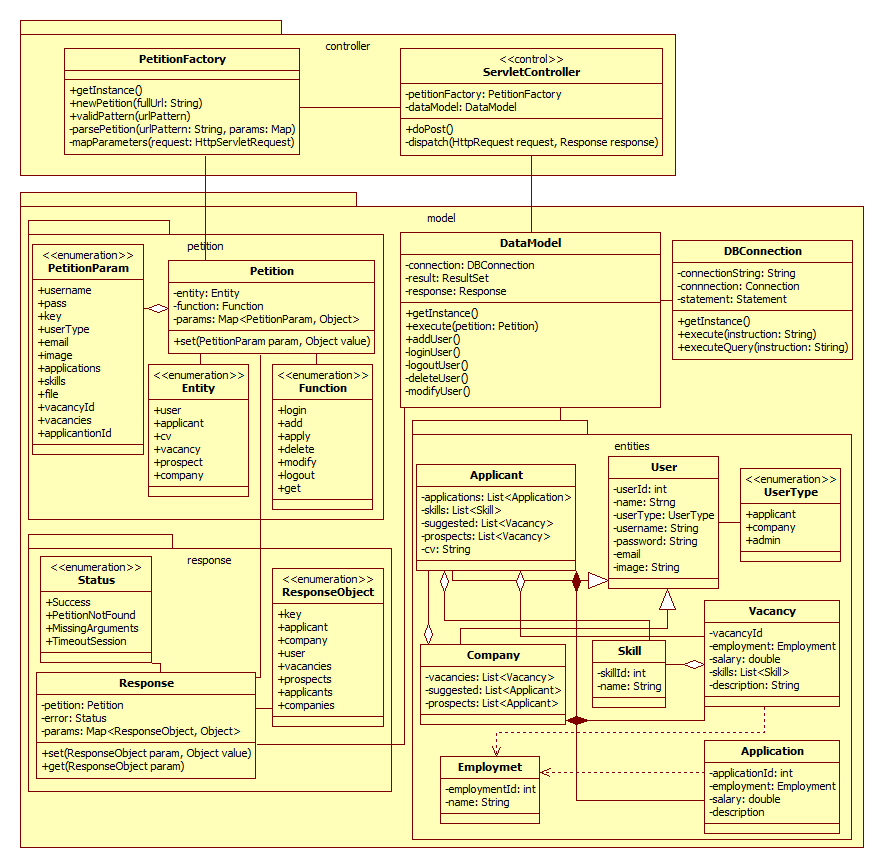
\includegraphics[scale=0.32]{./resources/ClassDiagram.png}
  \end{center}
}
\newpage
\section{Look \& Feel}
\frame
{
  \frametitle{ Look \& Fell, Ventana principal}
  \begin{center}
		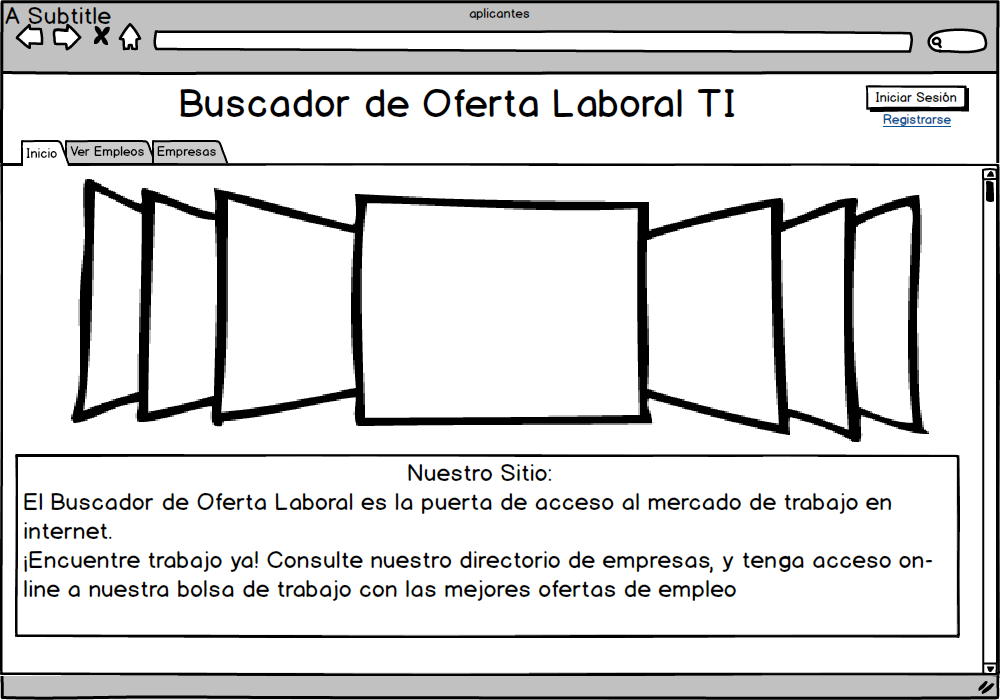
\includegraphics[scale=0.28]{./resources/02principal.png}
  \end{center}
}


\frame
{
  \frametitle{Registrarse}
  \begin{center}
		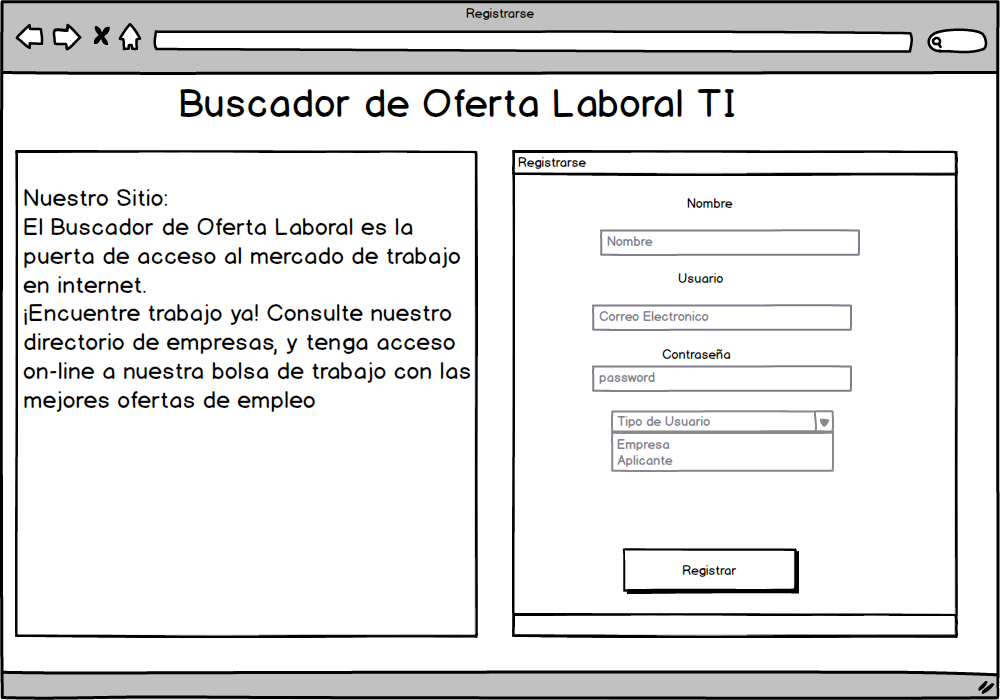
\includegraphics[scale=0.28]{./resources/01registrar.png}
  \end{center}
}

\frame
{
  \frametitle{  Ventana Inicio Sesión}
  \begin{center}
		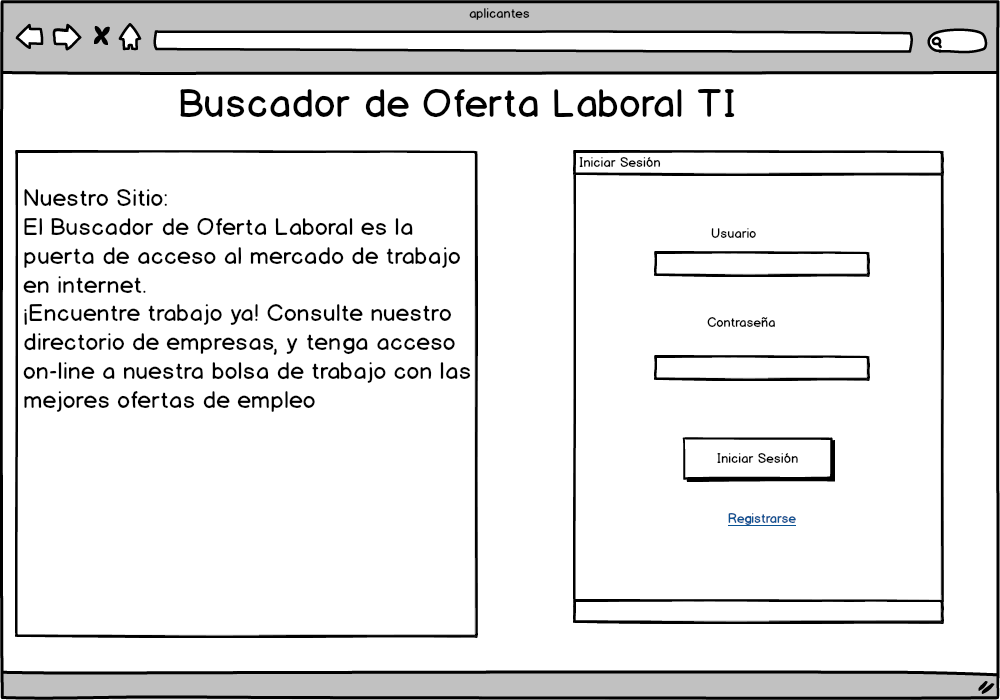
\includegraphics[scale=0.28]{./resources/04inicio.png}
  \end{center}
}


\frame
{
  \frametitle{  Ventana Perfil}
  \begin{center}
		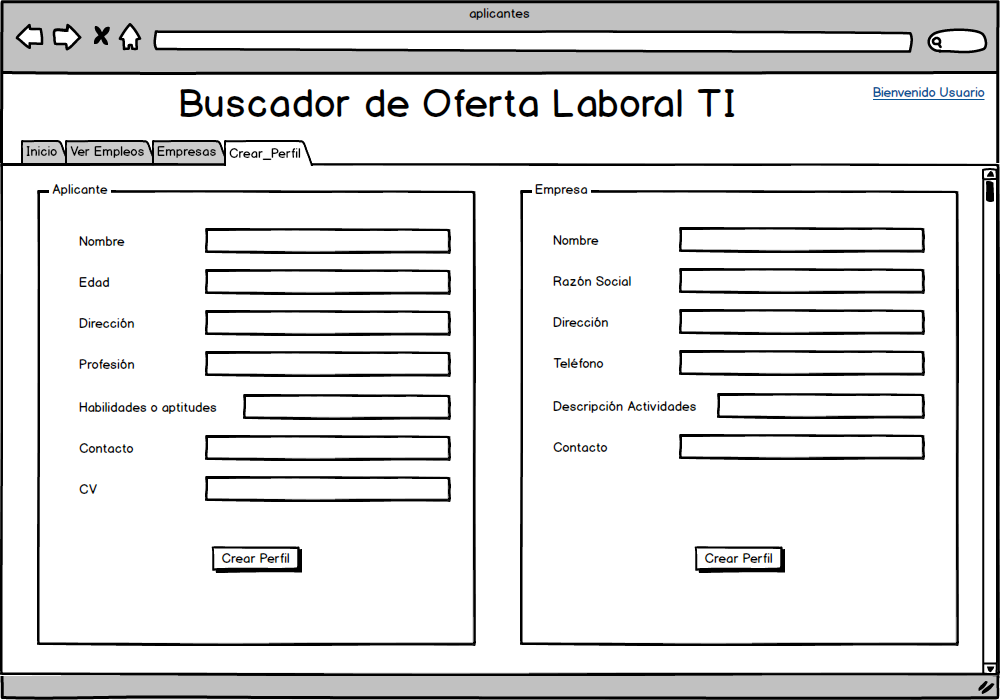
\includegraphics[scale=0.28]{./resources/06perfil.png}
  \end{center}
}

\frame
{
  \frametitle{  Ventana Sugeridos}
  \begin{center}
		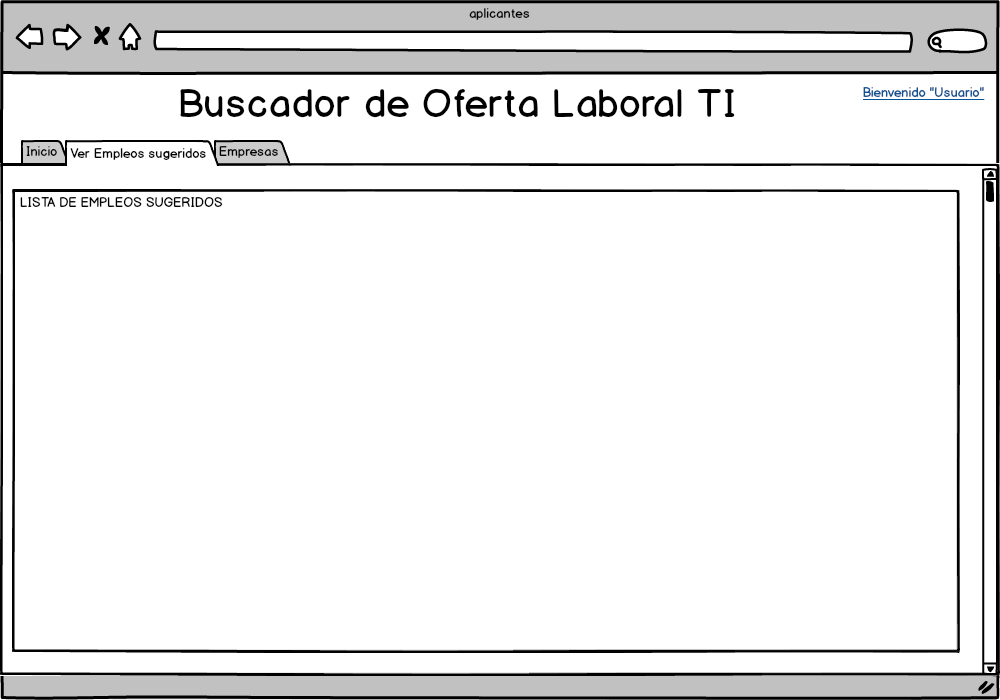
\includegraphics[scale=0.28]{./resources/08sugeridos.png}
  \end{center}
}

\frame
{
  \frametitle{  Ventana Cerrar cuenta}
  \begin{center}
		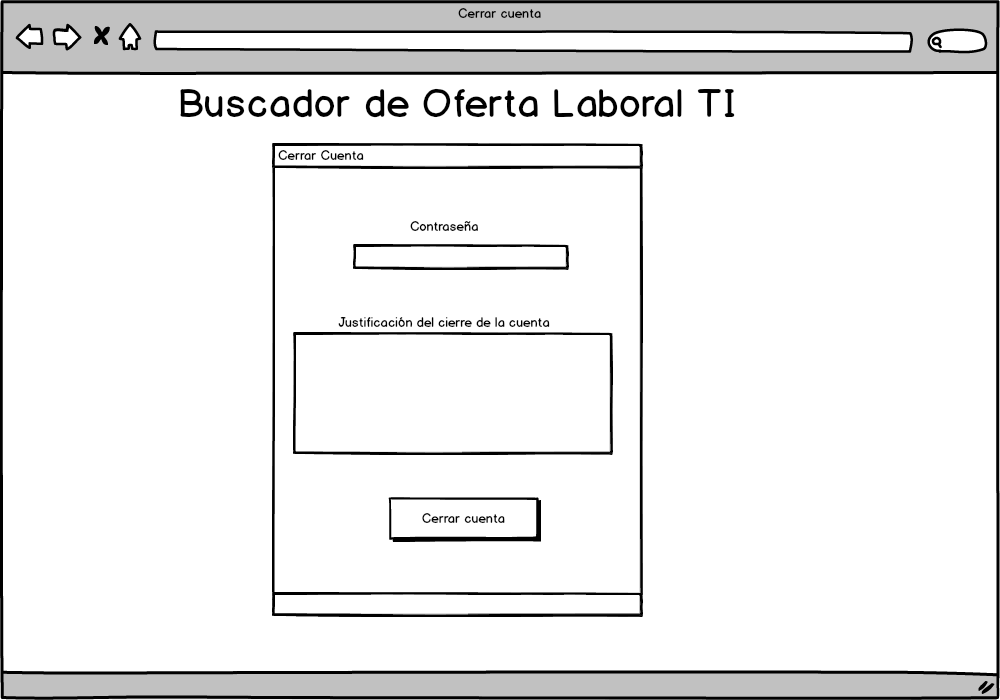
\includegraphics[scale=0.28]{./resources/09cerrarcuenta.png}
  \end{center}
}


\frame
{
  \frametitle{  Ventana Registro de Vacante}
  \begin{center}
		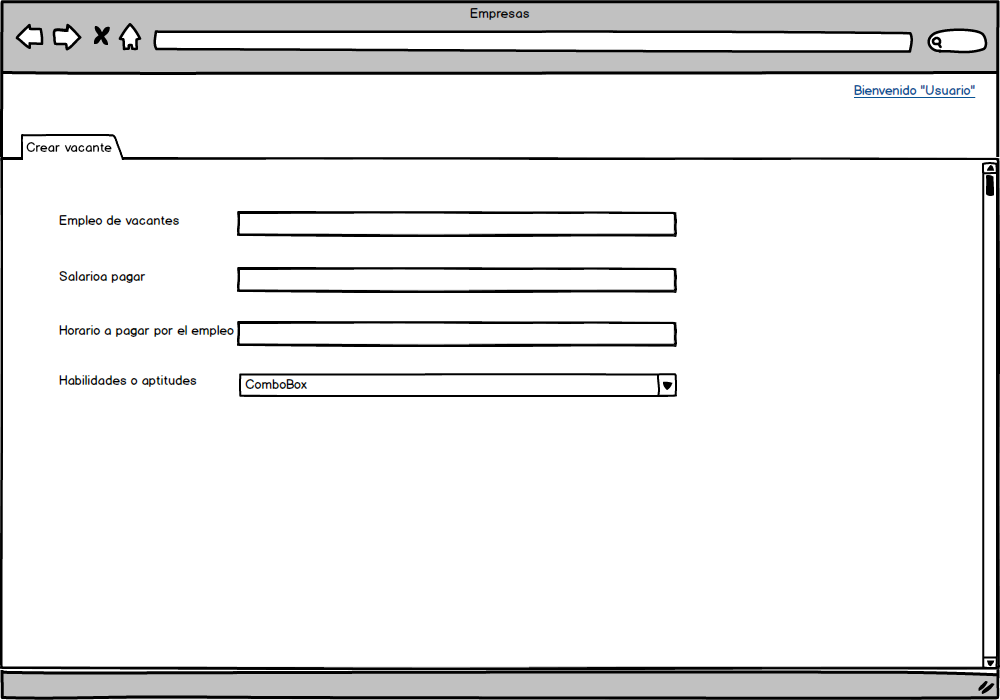
\includegraphics[scale=0.28]{./resources/13revacante.png}
  \end{center}
}


\frame
{
  \frametitle{  Ventana Ver aplicantes}
  \begin{center}
		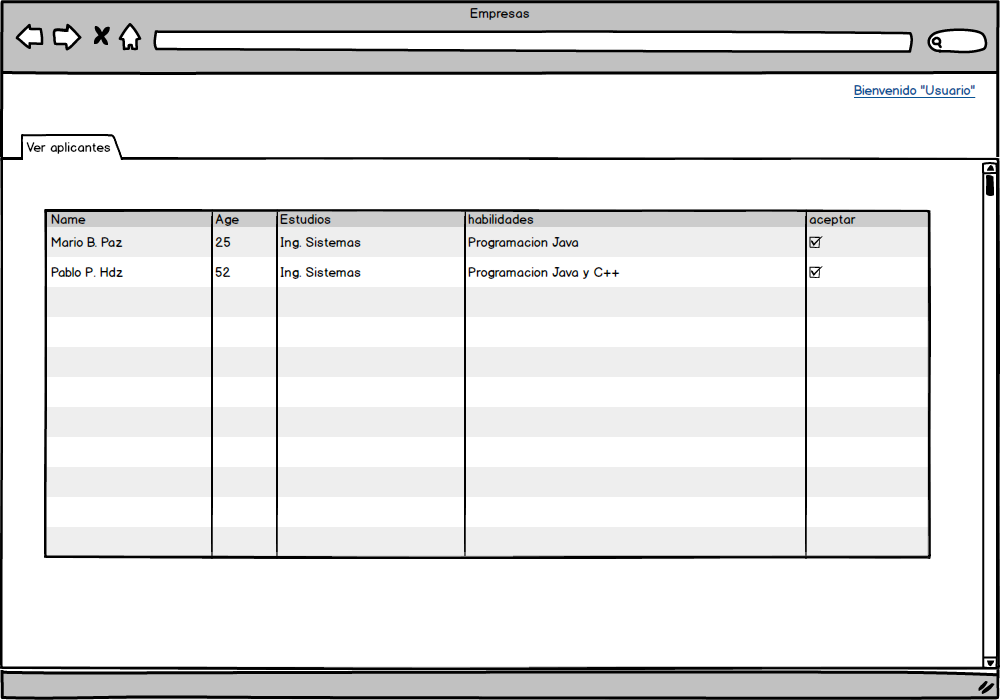
\includegraphics[scale=0.28]{./resources/14verapicantes.png}
  \end{center}
}

\frame
{
  \frametitle{  Ventana Administrador}
  \begin{center}
		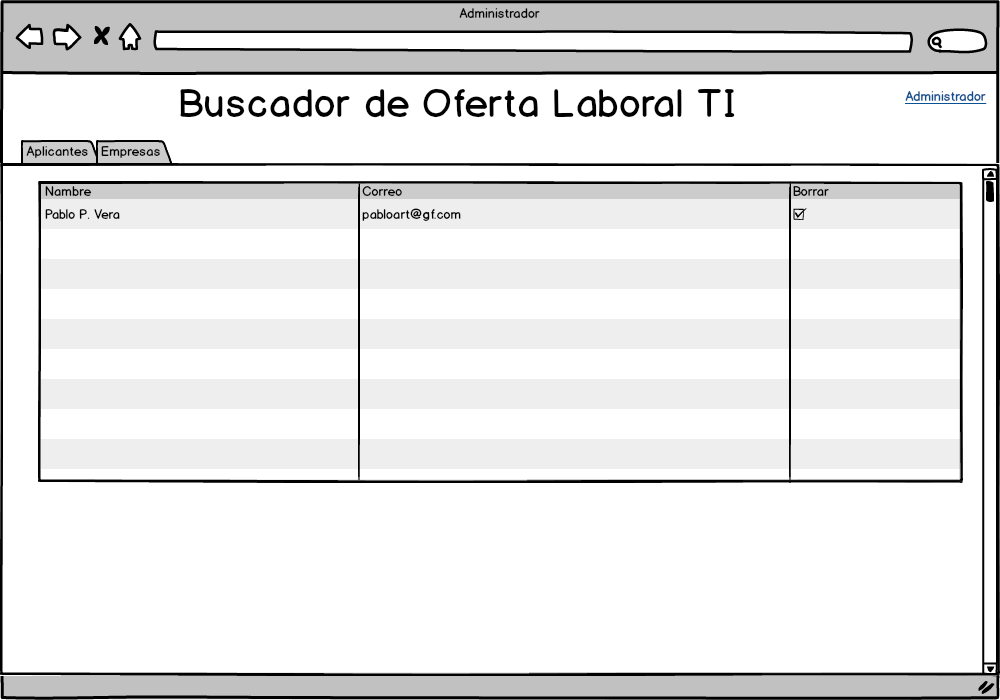
\includegraphics[scale=0.28]{./resources/15adm.png}
  \end{center}
}
\newpage
\section{Bibliografía} 
  \vspace{1 cm}

\begin{itemize}
	%\item  \textbf{Site name:: Topic title}, Author Name and Last Name, DD de MM de YYYY
	%\newline http://source-url.net/
	\item \textbf{[1]Empleo y Desempleo: Un ánalisis Socio-Psicológico}, Marie Ahoda. 1992, Ed. Morata 1986.
	\item \textbf{[2]WordReference.com:: Empleado}, 02 de Septiembre de 2013
	\newline http://www.wordreference.com/definicion/empleado
	
	\item \textbf{[3]Profeco.gob.mx:: Comercio Electrónico}, 02 de Septiembre de 2013
	\newline http://www.profeco.gob.mx/internacionales/com-elec.asp

\end{itemize}







	
\end{document}
